\chapter{Iterazione 2: Implementazione dell'Analytics Service}
\label{chap:iterazione2}

\section{Obiettivi e Ruolo Architetturale}

L'Iterazione 2 sposta il focus dalla gestione del dato (persistenza) alla sua elaborazione (intelligenza). L'obiettivo è la realizzazione dell'\textbf{Analytics Service}, un microservizio stateless progettato per utlizzare i dati grezzi forniti dall'Accounting Service e trasformarli in metriche finanziarie di alto livello.

A differenza del servizio precedente, qui la complessità non risiede nell'interazione con il database (assente in questo modulo), ma nella logica algoritmica di aggregazione e proiezione. Le sfide principali affrontate sono state:
\begin{itemize}
    \item L'implementazione di una comunicazione sincrona tra microservizi robusta e configurabile.
    \item La progettazione di algoritmi di aggregazione efficienti con complessità lineare $O(n)$.
    \item La garanzia della correttezza matematica dei calcoli finanziari tramite test isolati.
\end{itemize}

\section{Stack Tecnologico e Configurazione}

L'applicazione condivide lo stack base (Java 21, Spring Boot 3.2.0, Lombok) ma introduce componenti specifici per il suo ruolo di "Consumer".

\subsection{Configurazione del Client HTTP (RestTemplate)}
Per comunicare con l'Accounting Service, è stato scelto \textbf{RestTemplate}. Per evitare di istanziare manualmente l'oggetto in ogni classe (anti-pattern), è stato configurato come un Bean gestito dal container di Spring.

\bigskip

\begin{lstlisting}[language=Java, label={lst:resttemplate}]
@Configuration
public class RestTemplateConfig {
    @Bean
    public RestTemplate restTemplate() {
        return new RestTemplate();
    }
}
\end{lstlisting}
Questa scelta permette, in futuro, di iniettare configurazioni globali come timeout di connessione o intercettori per l'autenticazione, centralizzando la gestione della rete.

\subsection{Externalizzazione delle Dipendenze}
Un aspetto critico nei sistemi distribuiti è evitare di "scrivere nel codice" gli indirizzi IP o gli URL degli altri servizi (\textit{Hardcoding}).
Nel file \texttt{application.properties}, l'URL del servizio produttore è parametrizzato:

\bigskip

\begin{lstlisting}[language=bash, label={lst:props}]
server.port=8082
spring.application.name=analytics-service

# URL con valore di default, sovrascrivibile da variabili d'ambiente
accounting.service.url=${ACCOUNTING_SERVICE_URL:http://localhost:8081/api/transactions}
\end{lstlisting}
Questo approccio rispetta il principio III delle \textit{12-Factor App} (Config), permettendo di cambiare l'indirizzo del servizio Accounting (es. in un ambiente Docker o Kubernetes) senza ricompilare il jar.

\newpage

\section{Implementazione della Logica di Business}

Il cuore del servizio è la classe \texttt{AnalyticsService}. Analizziamo le decisioni implementative riga per riga.

\subsection{Modellazione dei Dati (Type Safety)}
Prima di eseguire calcoli, è stato necessario definire un contratto dati rigoroso.
L'uso di \texttt{BigDecimal} è stato confermato per tutti i campi monetari. Inoltre, per gestire la distinzione tra entrate e uscite, si è evitato l'uso di convenzioni fragili (come il segno meno) a favore di un Enum esplicito.

\bigskip

\begin{lstlisting}[language=Java, label={lst:enum}]
public enum TransactionType {
    INCOME,  // Entrata esplicita
    EXPENSE  // Uscita esplicita
}
\end{lstlisting}

\subsection{Algoritmo di Aggregazione (Design in Piccolo)}

Il metodo \texttt{generateReport()} implementa l'algoritmo principale. Il suo compito è trasformare una lista piatta di transazioni in un oggetto strutturato \texttt{FinancialReportDTO}.

\textbf{Fase 1: Fetching dei Dati}
Il servizio esegue una chiamata HTTP GET. L'array JSON ricevuto viene automaticamente deserializzato in un array di oggetti \texttt{TransactionDTO}.

\bigskip

\begin{lstlisting}[language=Java, label={lst:fetch}]
public FinancialReportDTO generateReport() {
    TransactionDTO[] response = restTemplate.getForObject(
        accountingUrl, TransactionDTO[].class);
    
    if (response == null || response.length == 0) {
        return new FinancialReportDTO(); // Oggetto vuoto (Pattern Null Object)
    }
    // ...
}
\end{lstlisting}

\newpage
\textbf{Fase 2: Scansione e Accumulo}
L'algoritmo itera sulla lista una sola volta. Per ogni transazione, verifica il tipo e aggiorna i contatori. Contestualmente, popola una \texttt{HashMap} per raggruppare le spese per categoria.

\bigskip

\begin{lstlisting}[language=Java, label={lst:algo_core}]
BigDecimal incomes = BigDecimal.ZERO;
BigDecimal expenses = BigDecimal.ZERO;
Map<String, BigDecimal> categories = new HashMap<>();

for (TransactionDTO t : transactions) {
    // Accumulo condizionale
    if (t.getType() == TransactionType.INCOME) {
        incomes = incomes.add(t.getAmount());
    } else if (t.getType() == TransactionType.EXPENSE) {
        expenses = expenses.add(t.getAmount());
        
        // Aggregazione per categoria: 
        // Se la chiave esiste somma, altrimenti inizializza
        categories.merge(t.getCategory(), t.getAmount(), BigDecimal::add);
    }
}
\end{lstlisting}

La scelta di usare \texttt{Map.merge} è stilisticamente e performantemente superiore a un blocco \texttt{if-contains-put}, rendendo il codice più conciso.

\section{Analisi dell'Algoritmo di Analytics}

Il cuore dell'Analytics Service è l'algoritmo di elaborazione finanziaria implementato nel metodo \texttt{generateReport}. Questo algoritmo non si limita a una semplice somma, ma esegue una pipeline di trasformazione dei dati divisa in due stadi logici:
\begin{enumerate}
    \item \textbf{Fase di Aggregazione (Iterativa)}: Scansione dello storico transazionale per il calcolo dei totali e il raggruppamento per categorie.
    \item \textbf{Fase di Proiezione e Valutazione (Analitica)}: Applicazione di modelli predittivi e logiche decisionali basate su soglie (Alert System).
\end{enumerate}

\subsection{Pseudocodice Formale}

Di seguito viene presentato lo pseudocodice completo dell'algoritmo, che evidenzia la complessità della logica di business implementata.

\bigskip

\begin{lstlisting}[mathescape=true, label={lst:pseudocode_analytics}]
Algoritmo GenerateFinancialReport(transactions[]):
    Input: Array $T$ di $N$ transazioni
    Output: Report $R$ con metriche e proiezioni

    // -- FASE 1: Aggregazione Lineare --
    Inizializza $Sum_{inc} \leftarrow 0$, $Sum_{exp} \leftarrow 0$
    Inizializza $Map_{cat} \leftarrow \emptyset$

    FOR each $t \in T$ DO:
        IF $t.type$ is INCOME THEN
            $Sum_{inc} \leftarrow Sum_{inc} + t.amount$
        ELSE IF $t.type$ is EXPENSE THEN
            $Sum_{exp} \leftarrow Sum_{exp} + t.amount$
            // Gestione collisioni e merge
            $Map_{cat}.merge(t.category, t.amount, SUM)$
        END IF
    END FOR

    // -- FASE 2: Proiezioni e Valutazione (calculateProjections) --
    $D_{cur} \leftarrow$ Giorno corrente del mese
    $D_{tot} \leftarrow$ Giorni totali nel mese corrente

    // Proiezione Spese (Linear Projection Model)
    IF $D_{cur} > 0$ THEN
        $Avg_{daily} \leftarrow Sum_{exp} / D_{cur}$
        $Proj_{month} \leftarrow Avg_{daily} \times D_{tot}$
    END IF

    // Valutazione Salute Finanziaria (Decision Tree)
    $Balance \leftarrow Sum_{inc} - Sum_{exp}$
    $SavingsRate \leftarrow 0$
    $Alert \leftarrow GRAY$

    IF $Sum_{inc} > 0$ THEN
        $SavingsRate \leftarrow (Balance / Sum_{inc}) \times 100$
        
        IF $SavingsRate > 20$ THEN $Alert \leftarrow GREEN$
        ELSE IF $SavingsRate > 0$ THEN $Alert \leftarrow YELLOW$
        ELSE $Alert \leftarrow RED$
    ELSE
        // Edge Case: Spese senza entrate
        IF $Sum_{exp} > 0$ THEN $Alert \leftarrow RED\_CRITICAL$
    END IF

    RETURN Report($Sum_{inc}, Sum_{exp}, Map_{cat}, Proj_{month}, Alert$)
\end{lstlisting}

\subsection{Analisi della Complessità Computazionale}

Per dimostrare l'efficienza e la scalabilità della soluzione, analizziamo il costo computazionale $T(n)$ in funzione del numero di transazioni $n$.

Il tempo totale di esecuzione è dato dalla somma dei costi delle due fasi:
\[ T(n) = T_{agg}(n) + T_{proj}(n) \]

\subsubsection{1. Costo della Fase di Aggregazione $T_{agg}(n)$}
Questa fase richiede l'iterazione su tutte le $n$ transazioni recuperate.
All'interno del ciclo, vengono eseguite le seguenti operazioni elementari:
\begin{itemize}
    \item \textbf{Type Checking}: Verifica del tipo di transazione ($O(1)$).
    \item \textbf{Aritmetica BigDecimal}: Le operazioni \texttt{add} su oggetti \texttt{BigDecimal} sono più costose delle primitive, dipendendo dalla precisione (numero di cifre significative $P$). Tuttavia, essendo la precisione fissata a 4 cifre decimali, possiamo considerare il costo costante $k_{math}$.
    \item \textbf{Aggiornamento HashMap}: L'operazione \texttt{merge} implica il calcolo dell'hash della categoria e l'accesso al bucket.
    \begin{itemize}
        \item Caso Medio: $O(1)$ (distribuzione uniforme delle chiavi).
        \item Caso Pessimo: $O(n)$ (tutte le chiavi collidono nello stesso bucket, degenerando in una lista linkata).
    \end{itemize}
\end{itemize}

Assumendo una buona funzione di hash, il costo della fase 1 è:
\[ T_{agg}(n) = \sum_{i=1}^{n} (c_{check} + k_{math} + c_{map}) \approx n \cdot C_1 \]
\[ T_{agg}(n) = O(n) \]

\subsubsection{2. Costo della Fase di Proiezione $T_{proj}(n)$}
Questa fase (metodo \texttt{calculateProjections}) non dipende dal numero di transazioni $n$, in quanto opera sui dati aggregati ($Sum_{inc}, Sum_{exp}$).
Esegue un numero fisso di operazioni matematiche complesse (divisioni con arrotondamento, moltiplicazioni) e valutazioni condizionali (IF/ELSE).
\[ T_{proj}(n) = C_2 \quad (\text{Costante}) \]
\[ T_{proj}(n) = O(1) \]

\subsubsection{Complessità Totale}
Combinando i risultati:
\[ T(n) = O(n) + O(1) \implies T(n) = O(n) \]

L'algoritmo presenta una \textbf{complessità lineare}. Questo è un risultato ottimale per un sistema di aggregazione, garantendo che il tempo di risposta cresca proporzionalmente al volume dei dati senza esplosioni esponenziali.

\subsection{Analisi della Complessità Spaziale}
Lo spazio di memoria richiesto $S(n)$ dipende principalmente dalla struttura dati utilizzata per il raggruppamento delle categorie.
Sia $K$ il numero di categorie uniche presenti nelle transazioni.
\[ S(n) = O(K) \]
Nel caso pessimo, in cui ogni transazione ha una categoria diversa, $K = n$, quindi $S(n) = O(n)$.
Tuttavia, nel dominio reale, il numero di categorie è limitato e molto inferiore al numero di transazioni ($K \ll n$), rendendo l'algoritmo efficiente anche in termini di memoria.

\newpage
\section{Algoritmi Predittivi e Sistema Esperto}

Oltre all'aggregazione, il servizio applica logiche di Business Intelligence.

\subsection{Proiezione Temporale (Stima a fine mese)}
Per calcolare la stima delle spese (\texttt{projectedMonthlyExpenses}), non è stata utilizzata una costante fissa (es. 30 giorni), ma la lunghezza esatta del mese corrente fornita da \texttt{java.time.LocalDate}.

\bigskip

\begin{lstlisting}[language=Java, label={lst:projection}]
LocalDate now = LocalDate.now();
int daysInMonth = now.lengthOfMonth(); // Es. 28, 30 o 31
int currentDay = now.getDayOfMonth();

BigDecimal dailyAverage = expenses.divide(
    BigDecimal.valueOf(currentDay), 2, RoundingMode.HALF_UP);
    
BigDecimal projection = dailyAverage.multiply(
    BigDecimal.valueOf(daysInMonth));
\end{lstlisting}

Questa attenzione al dettaglio ("Design for Accuracy") evita distorsioni nelle stime durante mesi particolari come Febbraio.

\subsection{Alert System (Savings Rate)}
Il calcolo del livello di allerta implementa una logica a soglie. Il codice gestisce anche i casi limite (divisione per zero se non ci sono entrate).

\bigskip

\begin{lstlisting}[language=Java, label={lst:alert}]
if (incomes.compareTo(BigDecimal.ZERO) > 0) {
    // Calcolo percentuale risparmio
    BigDecimal rate = balance.divide(incomes, 4, RoundingMode.HALF_UP)
                             .multiply(new BigDecimal("100"));

    if (rate.compareTo(new BigDecimal("20")) > 0) {
        report.setAlertLevel("GREEN - Ottimo risparmio");
        report.setFinancialAdvice("Ottimo lavoro! Continua a risparmiare cosi.");
    } else if (rate.compareTo(BigDecimal.ZERO) > 0) {
        report.setAlertLevel("YELLOW - Attenzione alle spese");
        report.setFinancialAdvice("Cerca di ridurre le spese non essenziali.");
    } else {
        report.setAlertLevel("RED - Bilancio in negativo!");
        report.setFinancialAdvice("Attenzione: le uscite superano le entrate.");
    }
} else {
    // Edge Case: Spese presenti ma zero entrate
    if (expenses.compareTo(BigDecimal.ZERO) > 0) {
        report.setAlertLevel("RED - Critical");
        report.setFinancialAdvice(" Attenzione! Stai spendendo senza alcuna entrata registrata.");
    }
}
\end{lstlisting}

\section{Qualità del Codice e Strategia di Testing}

Nell'Iterazione 2, il focus si è spostato sulla validazione di logiche di business complesse (aggregazioni, proiezioni) e sulla gestione delle dipendenze esterne. Essendo l'Analytics Service un consumatore di dati (tramite chiamate HTTP verso l'Accounting Service), la strategia di testing ha dovuto isolare queste dipendenze per garantire determinismo e affidabilità.

\subsection{Analisi della Complessità e Refactoring}

L'analisi statica iniziale ha evidenziato che il metodo principale \texttt{generateReport} presentava un'elevata \textbf{complessità cognitiva} a causa di logiche annidate per il calcolo delle proiezioni finanziarie.

Per migliorare la manutenibilità, sono stati applicati i seguenti interventi di refactoring:
\begin{itemize}
    \item \textbf{Estrazione della Logica:} Il calcolo delle proiezioni è stato isolato in metodi privati dedicati (es. \texttt{calculateProjections()}), riducendo la complessità ciclomatica del metodo principale.
    \item \textbf{Gestione delle Costanti:} Gli URL dei servizi e i parametri di soglia (es. "Magic Numbers" per gli alert) sono stati sostituiti con costanti \texttt{static final}, rendendo il sistema configurabile e meno soggetto a errori di battitura (Typos).
\end{itemize}

\begin{figure}[H]
    \centering
    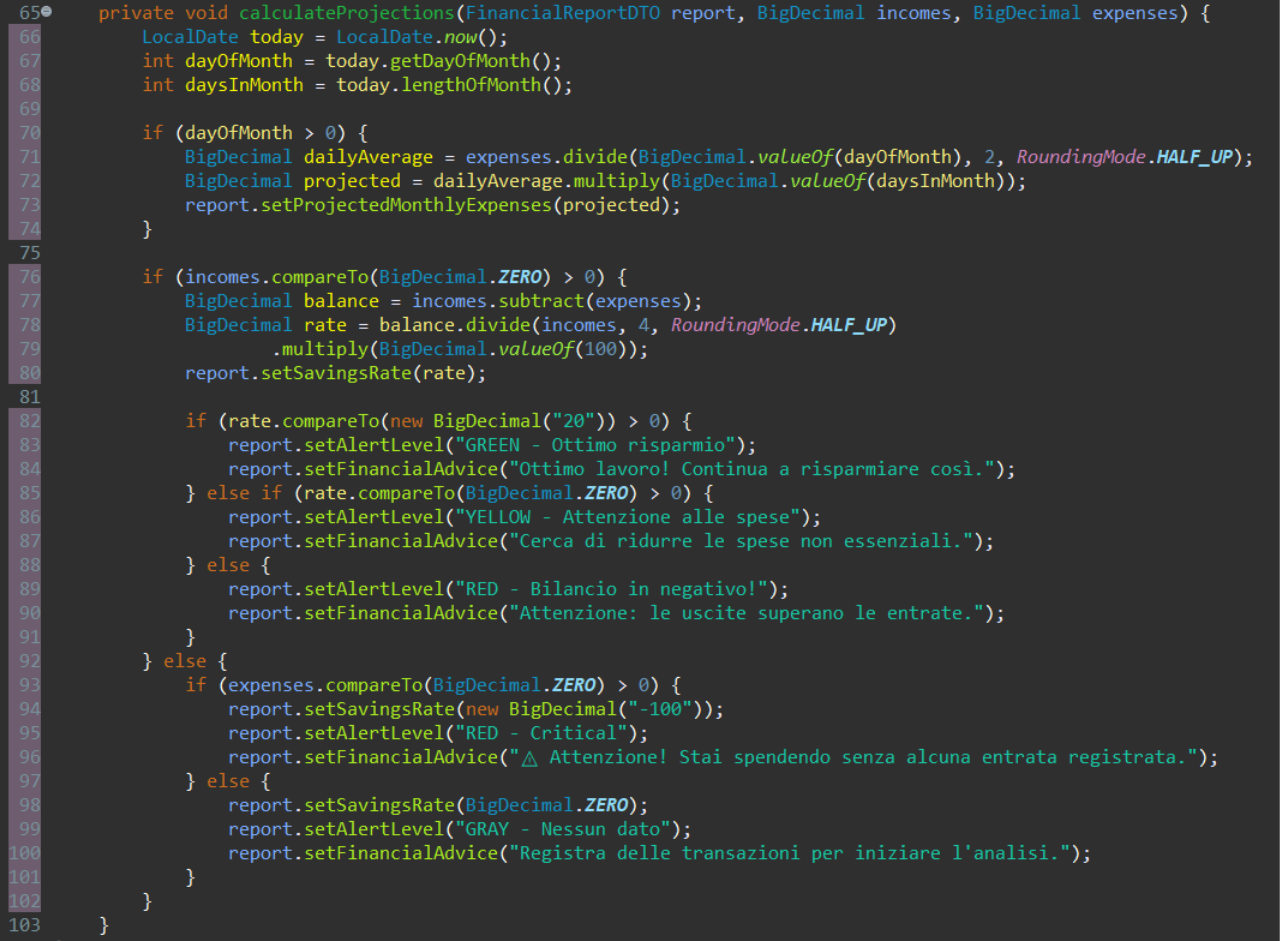
\includegraphics[width=0.9\textwidth]{../Iterazione_2/images/calculateProjections.png}
    \caption{Estrazione del metodo calculateProjections per ridurre la complessità}
    \label{fig:refactoring_projections}
\end{figure}

\section{Testing Isolato con Mockito}

Data la natura interconnessa del servizio, un semplice Unit Test non sarebbe sufficiente né affidabile se richiedesse l'istanza reale dell'Accounting Service attiva. Per garantire che i test siano deterministici e veloci, è stato utilizzato il framework \textbf{Mockito}.

La classe di test \texttt{AnalyticsServiceTest} utilizza le annotazioni:
\begin{itemize}
    \item \texttt{@Mock}: Crea una versione simulata di \texttt{RestTemplate}.
    \item \texttt{@InjectMocks}: Inietta il mock dentro l'istanza reale di \texttt{AnalyticsService}.
\end{itemize}

I test verificano la correttezza matematica dell'aggregatore e la logica degli alert (GREEN, RED, CRITICAL) fornendo dati fittizi tramite la tecnica dello "Stubbing".

Di seguito è riportato lo scenario "GREEN" (Risparmio positivo), dove si verifica che il calcolo del \textit{Savings Rate} e del \textit{Total Balance} sia corretto:

\begin{lstlisting}[language=Java, label={lst:mocktest}]
@Test
@DisplayName("Scenario GREEN: Entrate > Uscite (Risparmio Alto)")
void generateReport_GreenScenario() {
    // ARRANGE: Preparazione dati fittizi
    TransactionDTO income = new TransactionDTO();
    income.setAmount(new BigDecimal("2000.00"));
    income.setType(TransactionType.INCOME);

    TransactionDTO expense = new TransactionDTO();
    expense.setAmount(new BigDecimal("500.00"));
    expense.setType(TransactionType.EXPENSE);
    expense.setCategory("Svago");

    TransactionDTO[] mockResponse = {income, expense};

    // Istruiamo il Mock a restituire questi dati quando chiamato
    when(restTemplate.getForObject(any(), eq(TransactionDTO[].class)))
            .thenReturn(mockResponse);

    // ACT: Esecuzione reale del servizio
    FinancialReportDTO report = analyticsService.generateReport();

    // ASSERT: Verifica dei calcoli
    assertNotNull(report);
    assertEquals(new BigDecimal("1500.00"), report.getTotalBalance());
    assertEquals(new BigDecimal("75.0000"), report.getSavingsRate());
    
    // Verifica logica di business (Alert Level)
    assertTrue(report.getAlertLevel().contains("GREEN"));
}
\end{lstlisting}

\begin{figure}[H]
    \centering
    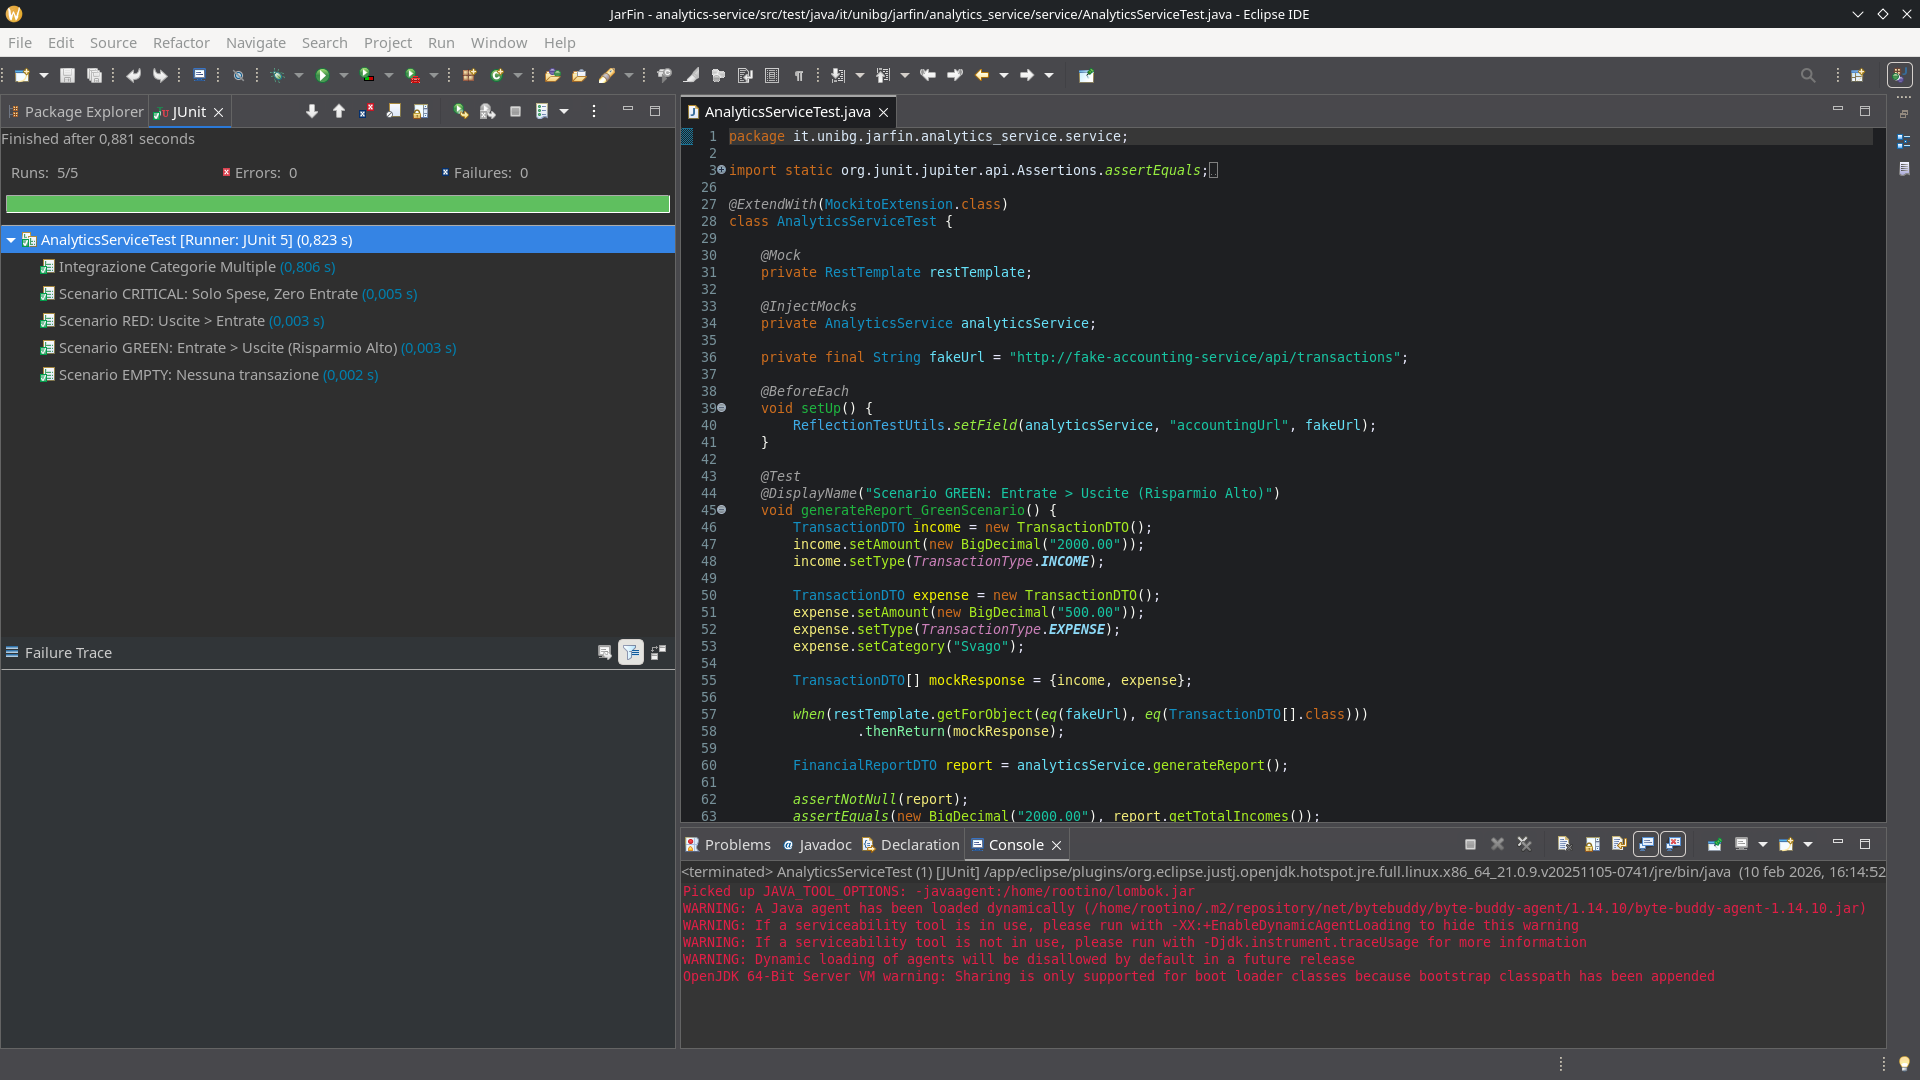
\includegraphics[width=0.9\textwidth]{../Iterazione_2/images/AnalyticsServiceTest.png}
    \caption{Esito positivo della suite di test.}
    \label{fig:junit_analytics}
\end{figure}

Questo approccio rispetta la piramide dei test, validando la logica di aggregazione e le regole di business senza dipendere dalla disponibilità della rete o del database.

\subsection{Metriche di Copertura e Qualità}

Anche per questo modulo è stato mantenuto l'approccio mirato al testing delle componenti critiche. Le metriche rilevate da \textbf{EclEmma} confermano un'alta copertura del codice:

\begin{itemize}
    \item \textbf{Service Layer Coverage:} 92\%
    \item \textbf{DTO Layer Coverage:} 100\%
    \item \textbf{Analytics Service Package Coverage:} 94.2\%
\end{itemize}

\begin{figure}[H]
    \centering
    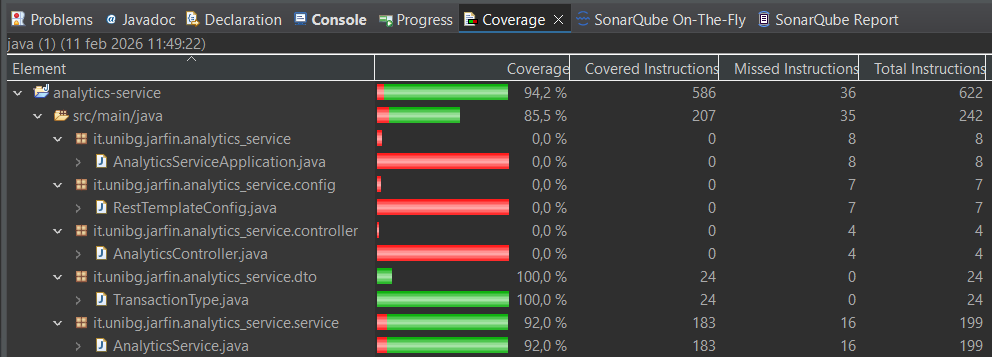
\includegraphics[width=0.8\textwidth]{../Iterazione_2/images/Ecl-analytics-service.png}
    \caption{Report di copertura EclEmma per il microservizio analytics-service}
    \label{fig:eclemma_analytics}
\end{figure}

L'analisi architetturale con \textbf{CodeMR} (Figura \ref{fig:codemr_analytics_quality}) evidenzia attributi di qualità positivi per il package, mentre il grafo delle dipendenze (Figura \ref{fig:codemr_analytics_deps}) mostra una struttura pulita con dipendenze minime verso l'esterno.

\begin{figure}[H]
    \centering
    
\includegraphics[width=0.75\textwidth]{../Iterazione_2/images/quality-attributes.png}
    \caption{Metriche degli attributi di qualità per analytics-service}
    \label{fig:codemr_analytics_quality}
\end{figure}

\begin{figure}[H]
    \centering
    
\includegraphics[width=0.75\textwidth]{../Iterazione_2/images/dependencies.png}
    \caption{Grafo delle dipendenze del package analytics-service}
    \label{fig:codemr_analytics_deps}
\end{figure}

\subsection{Validazione Funzionale del Servizio}

Una volta validata la logica unitaria, è stata eseguita una verifica funzionale avviando il microservizio.

\subsubsection{Avvio e Inizializzazione}
Come mostrato nel log di avvio (Figura \ref{fig:run_analytics}), il servizio viene inizializzato correttamente sulla porta \texttt{8082}, pronto per ricevere richieste e comunicare con l'Accounting Service.

\begin{figure}[H]
    \centering
    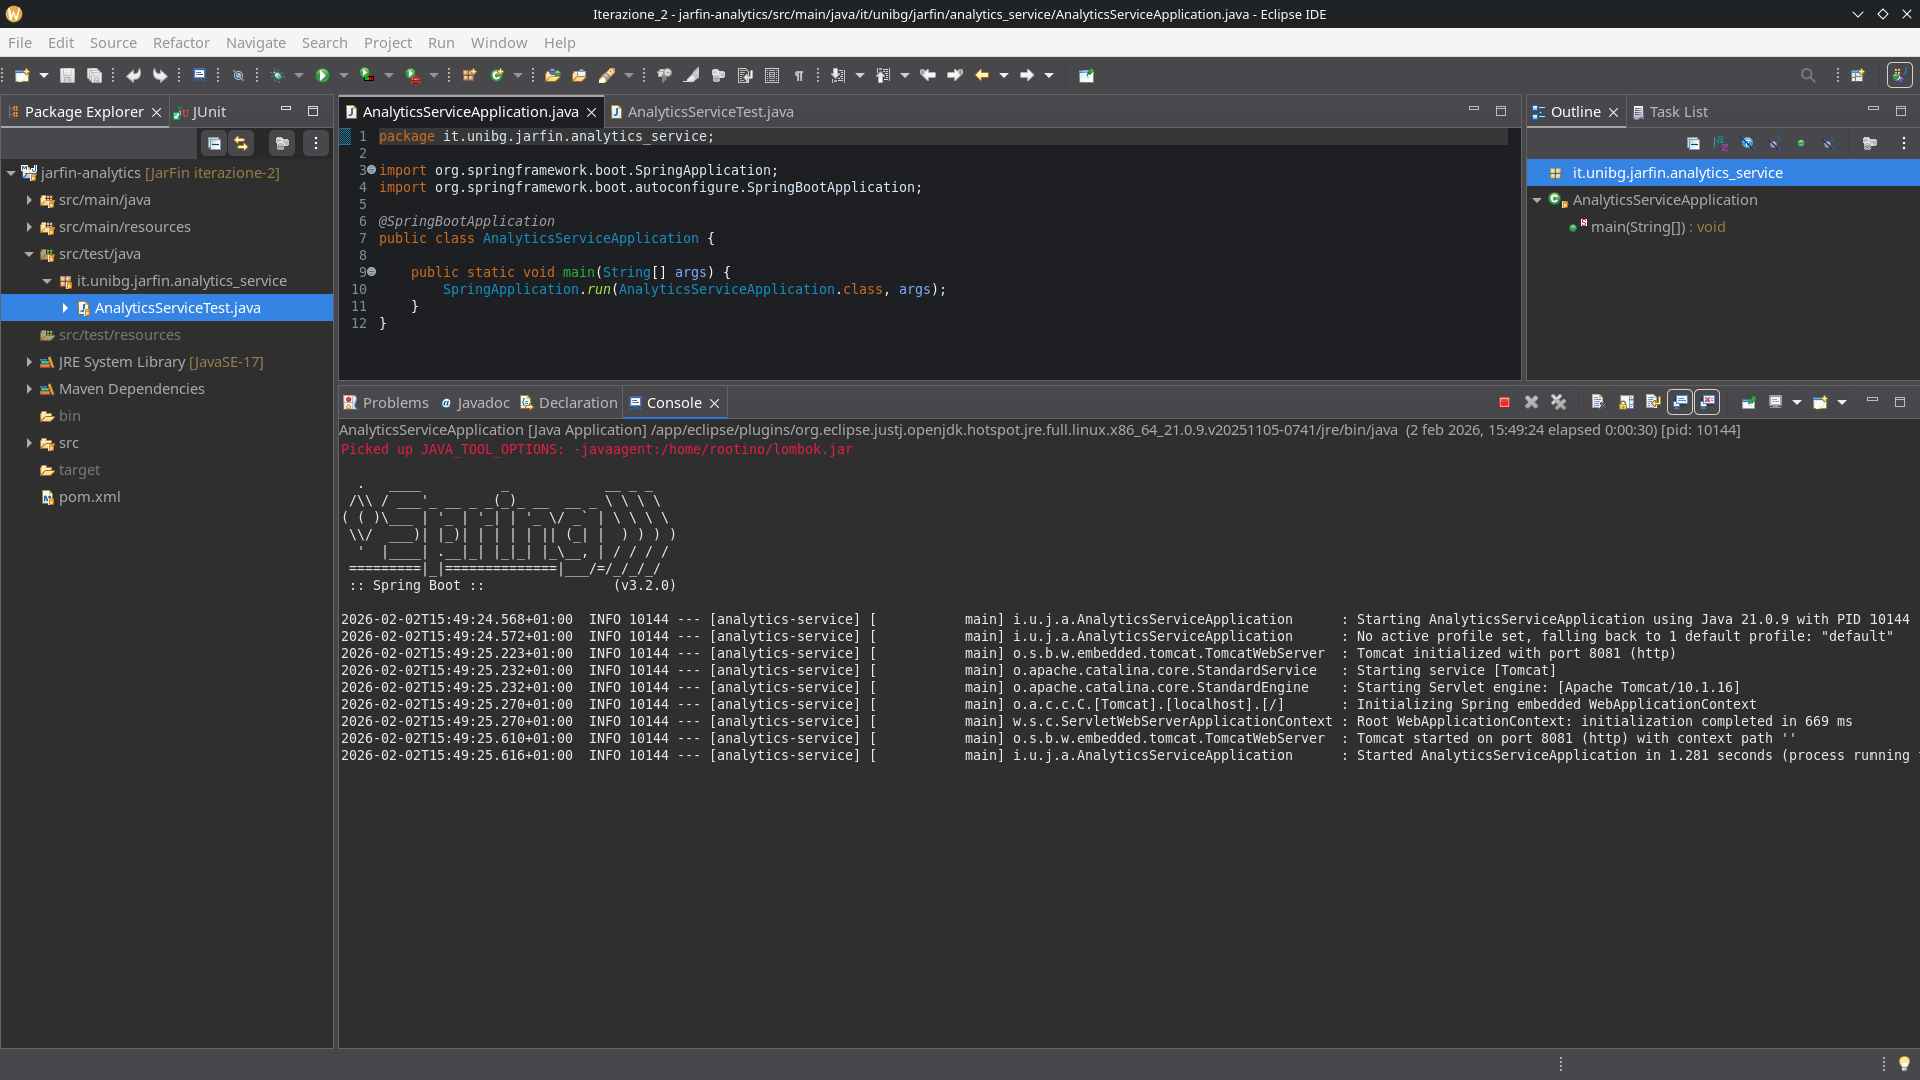
\includegraphics[width=0.9\textwidth]{../Iterazione_2/images/run_analytics_service.png}
    \caption{Console log: avvio di AnalyticsService sulla porta 8082}
    \label{fig:run_analytics}
\end{figure}

\subsubsection{Verifica Output JSON (Postman)}
Utilizzando Postman, è stata simulata una richiesta di report finanziario.
La risposta (Figura \ref{fig:postman_report}) dimostra che:
\begin{enumerate}
    \item I dati vengono recuperati correttamente dall'Accounting Service tramite la rete.
    \item L'algoritmo di aggregazione calcola correttamente i totali derivati (es. \texttt{totalBalance}, \texttt{totalExpenses}).
    \item Il sistema di alert funziona come previsto, restituendo un livello \texttt{GREEN} coerente con i dati di input (entrate superiori alle uscite oltre il margine di sicurezza).
\end{enumerate}

\begin{figure}[H]
    \centering
    
\includegraphics[width=0.9\textwidth]{../Iterazione_2/images/postman_get.png}
    \caption{Risposta JSON completa del report finanziario generato}
    \label{fig:postman_report}
\end{figure}

\section{Conclusione Iterazione 2}

L'Iterazione 2 ha prodotto un servizio di Analytics capace di elaborare dati complessi con efficienza. L'uso combinato di refactoring per ridurre la complessità cognitiva, mocking per i test unitari e analisi di copertura ha garantito un codice di alta qualità (copertura > 94\%). Le configurazioni externalizzate e i test isolati assicurano che il servizio sia pronto per l'integrazione nell'ecosistema containerizzato \textit{JarFin}.